
\chapter{Modello matematico per l'emodiafiltrazione}
Qui di seguito c'è la figura di riferimento per la trattazione matematica dell'HDF: è rappresentata l'interfaccia col paziente e i dettagli di ~pre- e ~post-diluizione.\\
\begin{figure}[htbp]
	\centering
		\includegraphics[width=0.90\textwidth]{immagini/modellofisico.eps}
	\caption{Modello fisico per l'HDF}
	\label{fig:modellofisico}
\end{figure}

Risolvendo i seguenti sistemi di equazioni è possibile calcolare la portata $Q_{inf}$ e la concentrazione del soluto $C_{inf}$ in ingresso al compartimento extracellulare del paziente.\\

\begin{equation}\label{sistinf}
	\left\{
		\begin{array}{l}
			Q_{inf} = Q_o+Q_{post}\\
			Q_{inf}C_{inf} = Q_oC_o + Q_{post}C_D
		\end{array}
	\right.
\end{equation}

\begin{equation}\label{sistout}
	\left\{
		\begin{array}{l}
			Q_o =Q_i-Q_F\\
			Q_oC_o =Q_iC_i-\Phi
		\end{array}
	\right.
\end{equation}

\begin{equation}\label{sistin}
	\left\{
		\begin{array}{l}
			Q_i =Q_{pre} + Q_b\\
			Q_iC_i =Q_bC_b + Q_{pre} C_D
		\end{array}
	\right.
\end{equation}
Il termine $\Phi$ cambia a seconda della modalità di depurazione del sangue, e in particolare vale:
\begin{equation*}
	\begin{cases}
	\Phi = \Phi_d & \text{per l'emodialisi,}\\
	\Phi = \Phi_{d_{HDF}} + \Phi_t & \text{per l'emodiafiltrazione,}\\
	\end{cases}
\end{equation*}
perché nel caso dell'emodialisi non vi è trasporto convettivo ma solo diffusivo, mentre nell'emodiafiltrazione ci sono entrambi; in più i valori dei flussi diffusivi non si calcolano allo stesso modo. Il calcolo di queste quantità è affrontato qui di seguito.\\

\section{Portata in massa di tipo diffusivo e  di tipo convettivo}
Indipendentemente dalla modalità di dialisi, emodialisi o emodiafiltrazione, la quantità di soluto eliminata nell'unità di tempo ($mmol/s$) dal dispositivo si può calcolare dal bilancio ingresso-uscita:\\
$$
\Phi = Q_i C_i - Q_o C_o
$$\\
Considerando ora che $Q_o = Q_i - Q_F$, riarrangiando i termini si ottiene:\\
\begin{equation}\label{general1}
\Phi = Q_i (C_i - C_o) + Q_F C_o
\end{equation}\\
La \textit{Dialisance} è definita, in assenza di ultrafiltrazione, come la \textit{variazione di soluto nel sangue in ingresso per unità di differenza di concentrazione fra compartimento sangue e dialisato utile alla diffusione}, ovvero:
\begin{equation*}
	D := \frac{Q_i(C_i-C_o)}{\alpha C_i - C_D}
\end{equation*}
dove $\alpha$ è il fattore di Donnan per il soluto alla membrana del dializzatore e $C_D$ è la concentrazione di soluto nel liquido dializzante. Alla luce di ciò possiamo riscrivere la (\ref{general1}) come:
\begin{equation}\label{general2}
	\Phi = D (\alpha C_i - C_D) + Q_F C_o
\end{equation}\\

\subsection{Emodialisi}
Ricaviamo ora $\Phi_d$ nel caso dell'emodialisi, ovvero quando $\Phi_t=0$.\\
Sostituendo nel sistema (\ref{sistout}) l'equazione (\ref{general2}) e $\Phi_t=0$ si ottiene:\\
\begin{equation}\label{coemo}
	C_o = C_i - \frac{D}{Q_i} (\alpha C_i - C_D)
\end{equation}\\
Nel caso dell'emodialisi $\Phi=\Phi_d$ perché è nullo il termine convettivo; sostituendo quindi la (\ref{coemo}) nella (\ref{general2}) otteniamo:
\begin{equation}\label{phidemo}
	\Phi_d = D (\alpha C_i - C_D)(1-\frac{Q_F}{Q_i}) + Q_F C_i
\end{equation}\\
In questa equazione il comparire del termine di trasporto $Q_F C_i$ non deve essere considerato come meccanimo fisico di trasporto; infatti nell'emodialisi il passaggio di soluto non avviene per convezione. Si tratta invece di un termine di trasporto matematico, che tiene conto dell'influenza dell'ultrafiltrazione sull'aumento delle concentrazioni a cavallo della membrana e di conseguenza dell'aumento della diffusione attraverso di essa.\\

\subsection{Emodiafiltrazione}
Nel caso dell'emodiafiltrazione (HDF) il termine $\Phi$ è pari alla somma di $\Phi_d$ e $\Phi_t$, ma questi ultimi due termini sono dipendenti l'uno dall'altro e dipendono emtrambi da $Q_F$, cioè:\\
\begin{equation}\label{phidf}
	\Phi(Q_F) = \Phi_d(Q_F,\Phi_t) + \Phi_t(Q_F,\Phi_d)
\end{equation}\\
Dai dati di letteratura si sa che quando i fenomeni di diffusione e trasporto avvengono contemporaneamente il flusso di soluto totale è inferiore al flusso dato dalla somma dei singoli processi presi singolarmente, ma superiore a entrambi.
In questa sede vogliamo ricavare una funzione $\Phi(Q_F)$ che tenga conto delle considerazioni appena esposte.\\
\begin{figure}[htbp]
	\centering
		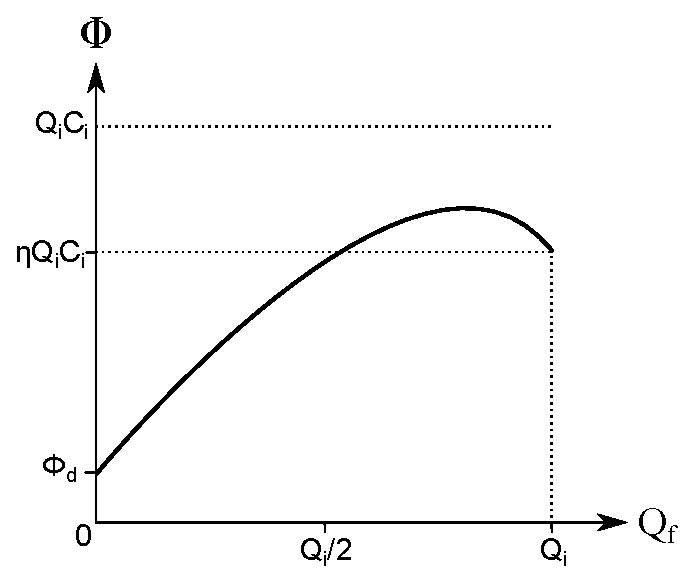
\includegraphics[width=0.70\textwidth]{immagini/hp_hdf.eps}
	\caption{ipotetica funzione per $\Phi(Q_F)$}
	\label{fig:PHI}
\end{figure}
La più semplice funzione per $\Phi$ è di tipo quadratica, in particolare ci si aspetta che si tratti di una parabola con la concavità verso il basso; una funzione di questo tipo infatti tiene conto dell'esistenza di un massimo fra i valori estremi che assume $Q_F$. La portata di ultrafiltrazione $Q_F$ varia da un minimo di zero a un massimo di $Q_i$: non è possibile infatti estrarre dal dializzatore più di quanto non vi entri. La funzione che vogliamo trovare è quindi:\\
\begin{equation}\label{phi}
		\Phi(Q_F) = aQ_F^2 + bQ_F + c  \text{,\qquad$Q_F$ $\in[0-Q_i]$}
\end{equation}\\
I coefficienti $a$, $b$ e $c$ li possiamo ricavare imponendo le condizioni al contorno:
\begin{subequations}\label{cc}
	\begin{align}
		&\Phi(0)=\Phi_d\label{cc0}\\
		&\Phi(Q_i)=Q_i C_i\label{cc1}\\
		&\frac{d\Phi}{dQ_F}\Biggr\rvert_{Q_F=0}=\frac{\partial\Phi_d}{\partial Q_F} + \frac{\partial\Phi_t}{\partial Q_F}\label{ccd}
	\end{align}
\end{subequations}
La condizione (\ref{cc0}) indica che in assenza di ultrafiltrazione il flusso $\Phi$ è puramente diffusivo e pari a (\ref{phidemo}); la condizione (\ref{cc1}) indica che flusso di soluto che si ottiene quando $Q_F$ è massimo è pari al flusso in ingresso al dializzatore; la condizione (\ref{ccd}) ha invece bisogno di una spiegazione un po' più lunga.\\
\newline
Considerando la (\ref{phidf}) e calcolandone il differenziale si ottiene:
\begin{equation}\label{diff}
	d\Phi = \frac{\partial \Phi_d}{\partial Q_F} dQ_F + \frac{\partial \Phi_d}{\partial \Phi_t} d\Phi_t
					+ \frac{\partial \Phi_t}{\partial Q_F} dQ_F + \frac{\partial \Phi_t}{\partial \Phi_d} d\Phi_d
\end{equation}
Possiamo ipotizzare che quando $Q_F\approxeq 0$ i flussi $\Phi_d$ e $\Phi_t$ sono indipendenti l'uno dall'altro; infatti in questa condizione il flusso trasportato per convezione è anche esso trascurabile e non influenza la variazione di concentrazione a cavallo della membrana utile alla diffusione; viceversa un eventuale passaggio di soluto per diffusione non influenza il flusso convettivo (\ref{phit}) poiché il soluto trasportato, essendo pari al valor medio $(C_i+C_D)/2$, resta invariato in quanto una diminuzione di $C_i$ è compensata da un aumento di pari entità di $C_D$.\\
\newline
Per le considerazioni ora fatte i termini ~$\partial \Phi_d/\partial \Phi_t$ e ~$\partial \Phi_t/\partial \Phi_d$ nella (\ref{diff}) possono considerarsi nulli. Quindi, con l'ipotesi di $Q_F$ trascurabile, la derivata del flusso totale di soluto rispetto alla portata di ultrafiltrazione è:\\
\begin{equation}\label{diff1}
	\frac{d\Phi}{dQ_F}\Biggr\rvert_{Q_F=0} = \frac{\partial \Phi_d}{\partial Q_F} + \frac{\partial \Phi_t}{\partial Q_F}
\end{equation}
Considerando la linearità dell'operatore di derivazione, la (\ref{diff1}) mostra chiaramente l'indipendenza reciproca di $\Phi_d$ e $\Phi_t$ e rende possibile l'applicazione del principio di \textit{sovrapposizione degli effetti}.\\
\newline
Le equazioni che a questo punto ci interessa derivare e calcolarne il valore per $Q_F=0$ sono:


	\begin{subequations}\label{phidt}
		\begin{align}
			&\Phi_d = D (\alpha C_i - C_D)(1-\frac{Q_F}{Q_i}) + Q_F C_i\\
			&\Phi_t = Q_F (1-\sigma) \frac{C_i+C_D}{2}\label{phit}
		\end{align}
	\end{subequations}
dove l'equazione per $\Phi_d$ è la stessa della (\ref{phidemo}); l'equazione per $\Phi_t$ mostra che la concentrazione trasportata è pari alla media del soluto a cavallo della membrana, ipotesi che deriva dal considerare la concentrazione del soluto linearmente variabile con lo spessore della membrana e prendendo il valore centrale e quindi medio, moltiplicata per il complemento a uno del coefficiente di riflessione $\sigma$ del soluto, considerando cioè solo le particelle che passano effettivamente la membrana. Le derivato sono:
\begin{subequations}\label{derphidt}
		\begin{align}
			&\frac{d\Phi_d}{dQ_F} = C_i -\frac{D}{Q_i}(\alpha C_i - C_D)\\
			&\frac{d\Phi_t}{dQ_F} = (1-\sigma)\frac{C_i+C_D}{2}
		\end{align}
	\end{subequations}
Le (\ref{derphidt}) sostituite nella (\ref{diff1}) esplicitano la condizione al contorno (\ref{ccd}).\\
\newline
A questo punto risolvendo la (\ref{phi}) con le condizioni al contorno (\ref{cc}) si ottengono i segueti valori per i coefficienti $a$, $b$ e $c$:\\
\begin{align*}
	a& = -\frac{1}{Q_i}(1-\sigma)\frac{C_i+C_D}{2}\\
	b& = C_i - \frac{1}{Q_i}D(\alpha C_i - C_D)+ (1-\sigma)\frac{C_i+C_D}{2}\\
	c& = D(\alpha C_i - C_D)
\end{align*}
Come anticipato il coefficiente $a$ è negativo, il che indica una parabola con la concavità verso il basso, in accordo coi dati sperimentali.\\
La formula per il flusso complessivo $\Phi$ in presenza contemporanea di dialisi e emofiltrazione è:
\begin{equation}\label{phihdf}
	\begin{split}
		\Phi_{tot_{HDF}}& = D(\alpha C_i - C_D)(1-\frac{Q_F}{Q_i})+Q_F C_i + Q_F(1-\sigma)\frac{C_i+C_D}{2}(1-\frac{Q_F}{Q_i})\\
		                & = \underbrace{D(\alpha C_i - C_D)(1-\frac{Q_F}{Q_i})+Q_F C_i - \frac{Q_F}{Q_i}\Phi_t}_{\Phi_{d_{HDF}}} + \Phi_t\\
		                & = \Phi_{d_{HDF}} + \Phi_t
	\end{split}
\end{equation}
La nuova quantità trovata, $\Phi_{d_{HDF}}$, è il flusso diffusivo corretto per la presenza di ultrafiltrazione e convezione. Per un ragionamento analogo a quello fatto per la (\ref{phidemo}) i termini convettivi che compaiono in $\Phi_{d_{HDF}}$ non sono flussi fisici, ma flussi matematici di correzione. Notiamo anche che per $\Phi_t=0$ ricadiamo nel caso dell'emodialisi.\\
\newline
Con la (\ref{phihdf}) è possibile trovare anche la condizione che massimizza il flusso. Imponendo nulla la derivata rispetto alla portata di ultrafiltrazione si ha:
\begin{equation*}
	\Phi_{tot_{HDF}}=\Phi_{max} \Leftrightarrow Q_F = \frac{C_iQ_i-D(\alpha C_i-C_D)}{(1-\sigma)(C_i+C_D)}+\frac{Q_i}{2}
\end{equation*}
Degno di nota è il fatto che indipendentemente dal soluto considerato, la condizione di flusso massimo si realizza per portate di ultrafiltrazione grandi almeno la metà della portata di ingresso.\\
